% !TeX program = lualatex
% =====================================================================
%  Master's Thesis Defense  ·  Generic QLBM with Boundary Conditions
%  Andrei-Daniel Tavă
%
%  BUILD: compiles with LuaLaTeX, XeLaTeX, or pdfLaTeX (fonts adapt).
%  Recommended:
%      latexmk -lualatex defense.tex
%
%  SPEAKER NOTES: every frame carries the spoken script in \note{}.
%    To project them on a second screen, uncomment ONE of:
%      \setbeameroption{show notes}                       % notes interleaved
%      \setbeameroption{show notes on second screen=right}% presenter view
%
%  Slides are intentionally minimal; the narration lives in the notes.
%  The talk targets ~7 min; the 1D demo (~2-3 min) is separate.
% =====================================================================
\documentclass[aspectratio=169,11pt]{beamer}

% ---- Fonts: adapt to the engine (pdfLaTeX / LuaLaTeX / XeLaTeX) ----
\usepackage{iftex}
\ifPDFTeX
  \usepackage[T1]{fontenc}
  \usepackage[utf8]{inputenc}
  \usepackage{lmodern}
\else
  \usepackage{fontspec}
  \setsansfont{Latin Modern Sans}
  \setmainfont{Latin Modern Roman}
  \setmonofont{Latin Modern Mono}
\fi

% ---- Math, quantum notation, figures ----
\usepackage{amsmath,amssymb}
\usepackage{braket}
\usepackage{tikz}
\usetikzlibrary{arrows.meta}
\usepackage{quantikz}
\usepackage{booktabs}

\graphicspath{{../src/img/figures/}{../src/img/branding/}}

% ---- Notes off by default (see header to enable) ----
%\setbeameroption{show notes}
%\setbeameroption{show notes on second screen=right}

% =====================================================================
%  Clean flat (metropolis-style) look, built from stock beamer
% =====================================================================
\usetheme{default}
\usefonttheme{professionalfonts}
\setbeamertemplate{itemize items}[square]
\setbeamertemplate{blocks}[default]

\definecolor{mDarkTeal}{RGB}{34,54,68}
\definecolor{mOrange}{RGB}{235,129,27}
\definecolor{mGreen}{RGB}{20,131,123}
\definecolor{mGray}{RGB}{120,120,120}

\setbeamercolor{normal text}{fg=mDarkTeal}
\setbeamercolor{structure}{fg=mDarkTeal}
\setbeamercolor{alerted text}{fg=mOrange}
\setbeamercolor{example text}{fg=mGreen}
\setbeamercolor{frametitle}{fg=white,bg=mDarkTeal}
\setbeamercolor{title}{fg=mDarkTeal}
\setbeamercolor{subtitle}{fg=mOrange}
\setbeamercolor{itemize item}{fg=mOrange}
\setbeamercolor{footline}{fg=mGray,bg=white}

\setbeamerfont{title}{series=\bfseries,size=\LARGE}
\setbeamerfont{frametitle}{series=\bfseries}

% Flat title bar
\setbeamertemplate{frametitle}{%
  \nointerlineskip%
  \begin{beamercolorbox}[wd=\paperwidth,sep=8pt]{frametitle}%
    \strut\insertframetitle\strut%
  \end{beamercolorbox}%
}

% No navigation symbols.
\setbeamertemplate{navigation symbols}{}

% Footer: short title · frame number
\setbeamertemplate{footline}{%
  \hbox{%
    \begin{beamercolorbox}[wd=\paperwidth,ht=3ex,dp=1.6ex,leftskip=8pt,rightskip=8pt]{footline}%
      {\tiny\insertshorttitle}%
      \hfill
      {\tiny\insertframenumber}%
    \end{beamercolorbox}%
  }%
}

% =====================================================================
%  Title metadata
% =====================================================================
\title[Generic QLBM with Boundary Conditions]{Generic Quantum Lattice Boltzmann Method}
\subtitle{with Boundary Conditions for Arbitrary Velocity Sets}
\author{Andrei-Daniel Tav\u{a}\\[2pt]{\small Adviser: Prof.\ Emil-Ioan Slu\c{s}anschi}}
\institute{Quantum Computing MSc\\National University of Science and Technology POLITEHNICA Bucharest}
\date{Master's Thesis Defense \,\textperiodcentered\, 2026}
\titlegraphic{
\includegraphics[height=1.3cm]{mscqc}}

\begin{document}

% =====================================================================
%  Title
% =====================================================================
\begin{frame}[plain]
  \titlepage
  \note{Hello dear colleagues, esteemed professors and all audience members.
  My name is Andrei and today I will present a little bit of my past two years of
  tackling a quantum algorithm for computational fluid dynamics.}
\end{frame}

% =====================================================================
%  Background
% =====================================================================
\section{Background}

\begin{frame}{Computational Fluid Dynamics}
  \vfill
  \centering
  \large
  Simulating fluids with computers.\\[1em]
  Complex, often run on supercomputers.\\[1em]
  {\color{mOrange} Can quantum computing help?}
  \vfill
  \note{To start off, a little bit of background: computational fluid dynamics, or CFD
  for short, is the field concerned with simulating fluids using computers. Modern CFD
  simulations can be very complex and usually require powerful supercomputers, so
  naturally any performance improvements would be incredible. With that in mind, trying
  to apply quantum computing to this field is worth a look.}
\end{frame}

\begin{frame}{Quantum Lattice Boltzmann Method}
  \vfill
  \centering
  My focus: the Quantum Lattice Boltzmann Method, applied to the\\
  \emph{Advection-Diffusion equation}.
  \[ \frac{\partial \Phi}{\partial t} = D\,\nabla^{2}\Phi - \nabla\cdot(\mathbf{u}\,\Phi) \]
  {\small Simpler than Navier-Stokes; models e.g.\ pollutant transport in air or water.}
  \vfill
  \note{There were several approaches to quantum algorithms for CFD that I found in the
  literature, but my focus has been the Quantum Lattice Boltzmann.}
\end{frame}

\begin{frame}{The Lattice Boltzmann Method}
  \centering
  \vspace{0.4em}
  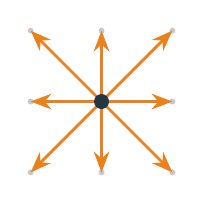
\begin{tikzpicture}[scale=0.9,>=Stealth,line width=1pt]
    \foreach \x in {-1,0,1}\foreach \y in {-1,0,1}{\fill[mGray!40] (\x,\y) circle (1.2pt);}
    \foreach \dx/\dy in {1/0,-1/0,0/1,0/-1,1/1,1/-1,-1/1,-1/-1}{\draw[->,mOrange] (0,0)--(\dx,\dy);}
    \fill[mDarkTeal] (0,0) circle (3pt);
  \end{tikzpicture}
  \\[0.6em]
  {\small Lattice $+$ discrete links; density split into populations.}
  \\[1em]
  \large Collision \;$\rightarrow$\; Streaming \;$\rightarrow$\; Summation
  \note{A very quick primer on the classical Lattice Boltzmann Method. Space is discretized
  into a lattice and velocity into a set of discrete links. The fluid density, or other
  physical quantity, is split between populations for each link and evolved via alternating
  collision and streaming steps. The final macroscopic quantity is obtained by summation.}
\end{frame}

\begin{frame}{Quantum encoding}
  \vfill
  \centering
  Density field $\rightarrow$ amplitudes of a quantum state:
  \[ \ket{\psi} \;\propto\; \sum_{x} \Phi(x)\,\ket{x} \]
  {\small The standard encoding; the idea is to exploit quantum parallelism.}
  \vfill
  \note{There is a bit of flexibility in choosing how to translate this algorithm to a
  quantum circuit, but I opted for what has by now become the standard encoding preferred
  by most research teams. The density field is encoded as the amplitudes of a quantum
  state, the main idea being to make use of quantum parallelism.}
\end{frame}

\begin{frame}{Collision is not unitary}
  \begin{columns}[c]
    \begin{column}{0.5\textwidth}
      \centering
      The collision operator is non-unitary.\\[0.8em]
      Apply it via a\\\emph{Linear Combination of Unitaries}:
      \[ M=\tfrac12\big(U_0+U_1\big) \]
      {\small One ancilla qubit; a measurement can land in the unwanted substate.}
    \end{column}
    \begin{column}{0.5\textwidth}
      \centering
      \begin{quantikz}[column sep=10pt,row sep=14pt]
        \lstick{$\ket{0}$} & \gate{H} & \octrl{1} & \ctrl{1} & \gate{H} & \meter{} \\
        \lstick{$\ket{\psi}$} & \qw & \gate{U_0} & \gate{U_1} & \qw & \qw
      \end{quantikz}
    \end{column}
  \end{columns}
  \note{Unfortunately the collision operator is not generally unitary. To fix this we can
  use a technique called Linear Combination of Unitaries, or LCU. We use an additional
  ancilla qubit, and this allows us to apply the original non-unitary matrix in one of the
  substates. This comes with the cost of having a chance to measure the non-desired
  substate at the end of the circuit.}
\end{frame}

\begin{frame}{Reading the result}
  \vfill
  \centering
  \large
  Recovering the macroscopic quantity needs \emph{all} amplitudes.
  \\[1em]
  Quantum State Tomography \;$\rightarrow$\; many circuit shots.
  \vfill
  \note{Lastly, to recover the macroscopic quantity, we need all coefficients of the
  quantum state. This is done via something called quantum state tomography and, without
  getting into details now, it requires a lot of shots of the circuit. I will get back to
  this later.}
\end{frame}

% =====================================================================
%  Contributions
% =====================================================================
\section{Contributions}

\begin{frame}[plain]
  \vfill
  \centering
  {\usebeamercolor[fg]{title}\Huge\bfseries Contributions}
  \vfill
  \note{With the background out of the way, let's get into my work.}
\end{frame}

\begin{frame}{One iteration as a quantum circuit}
  \vfill
  \centering
  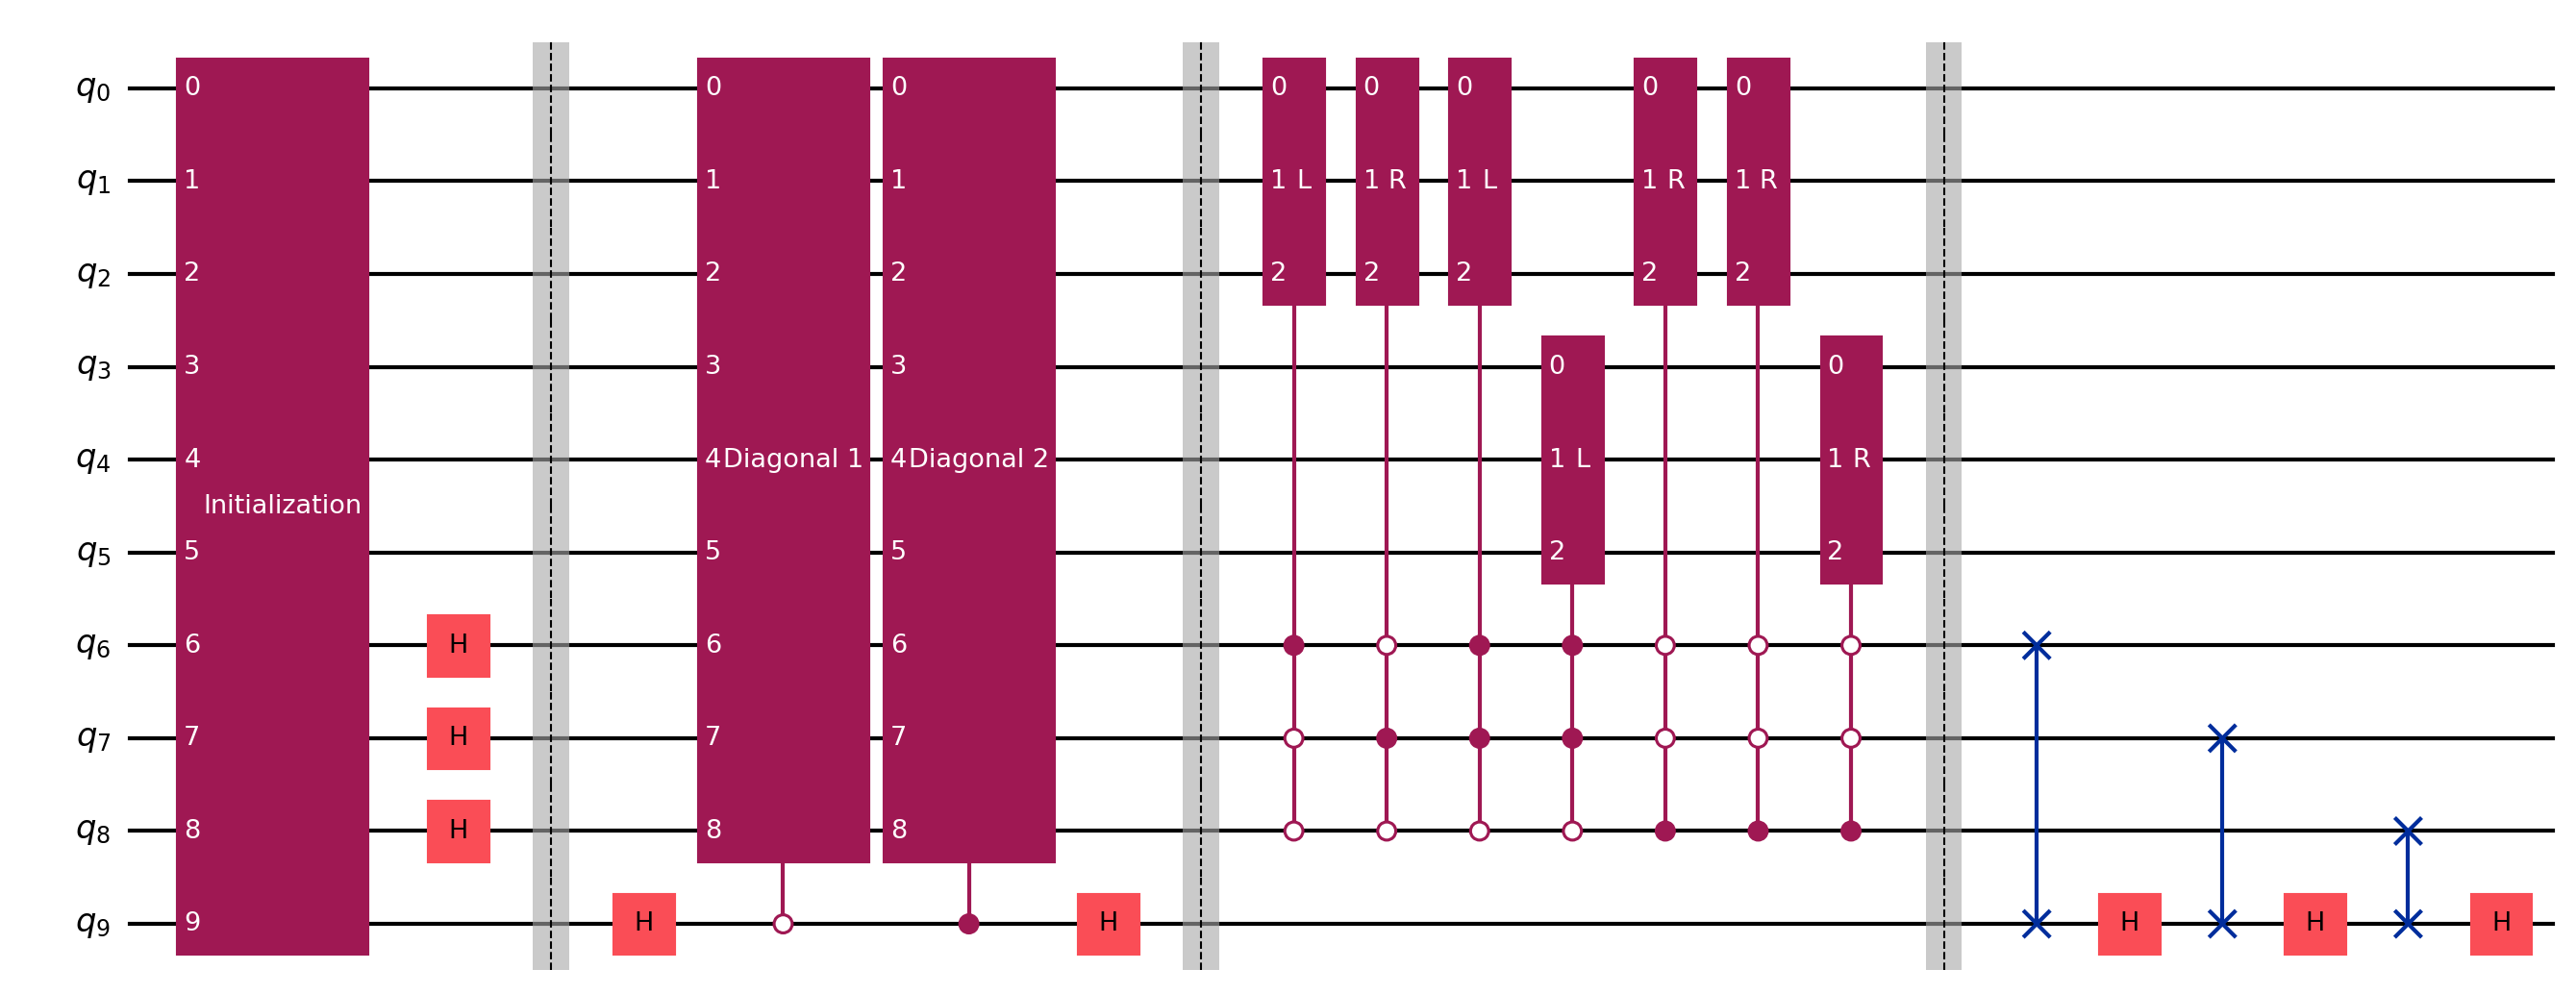
\includegraphics[width=\textwidth]{complete_circuit}
  \\[0.6em]
  {\small Initialization, collision (LCU), streaming, and macroscopic readout.}
  \vfill
  \note{First off, I have implemented the algorithm using a quantum circuit simulator. The
  algorithm itself is from the existing literature, with my contributions being
  implementation-side at best.}
\end{frame}

\begin{frame}{Validation}
  \begin{columns}[c]
    \begin{column}{0.5\textwidth}
      \centering
      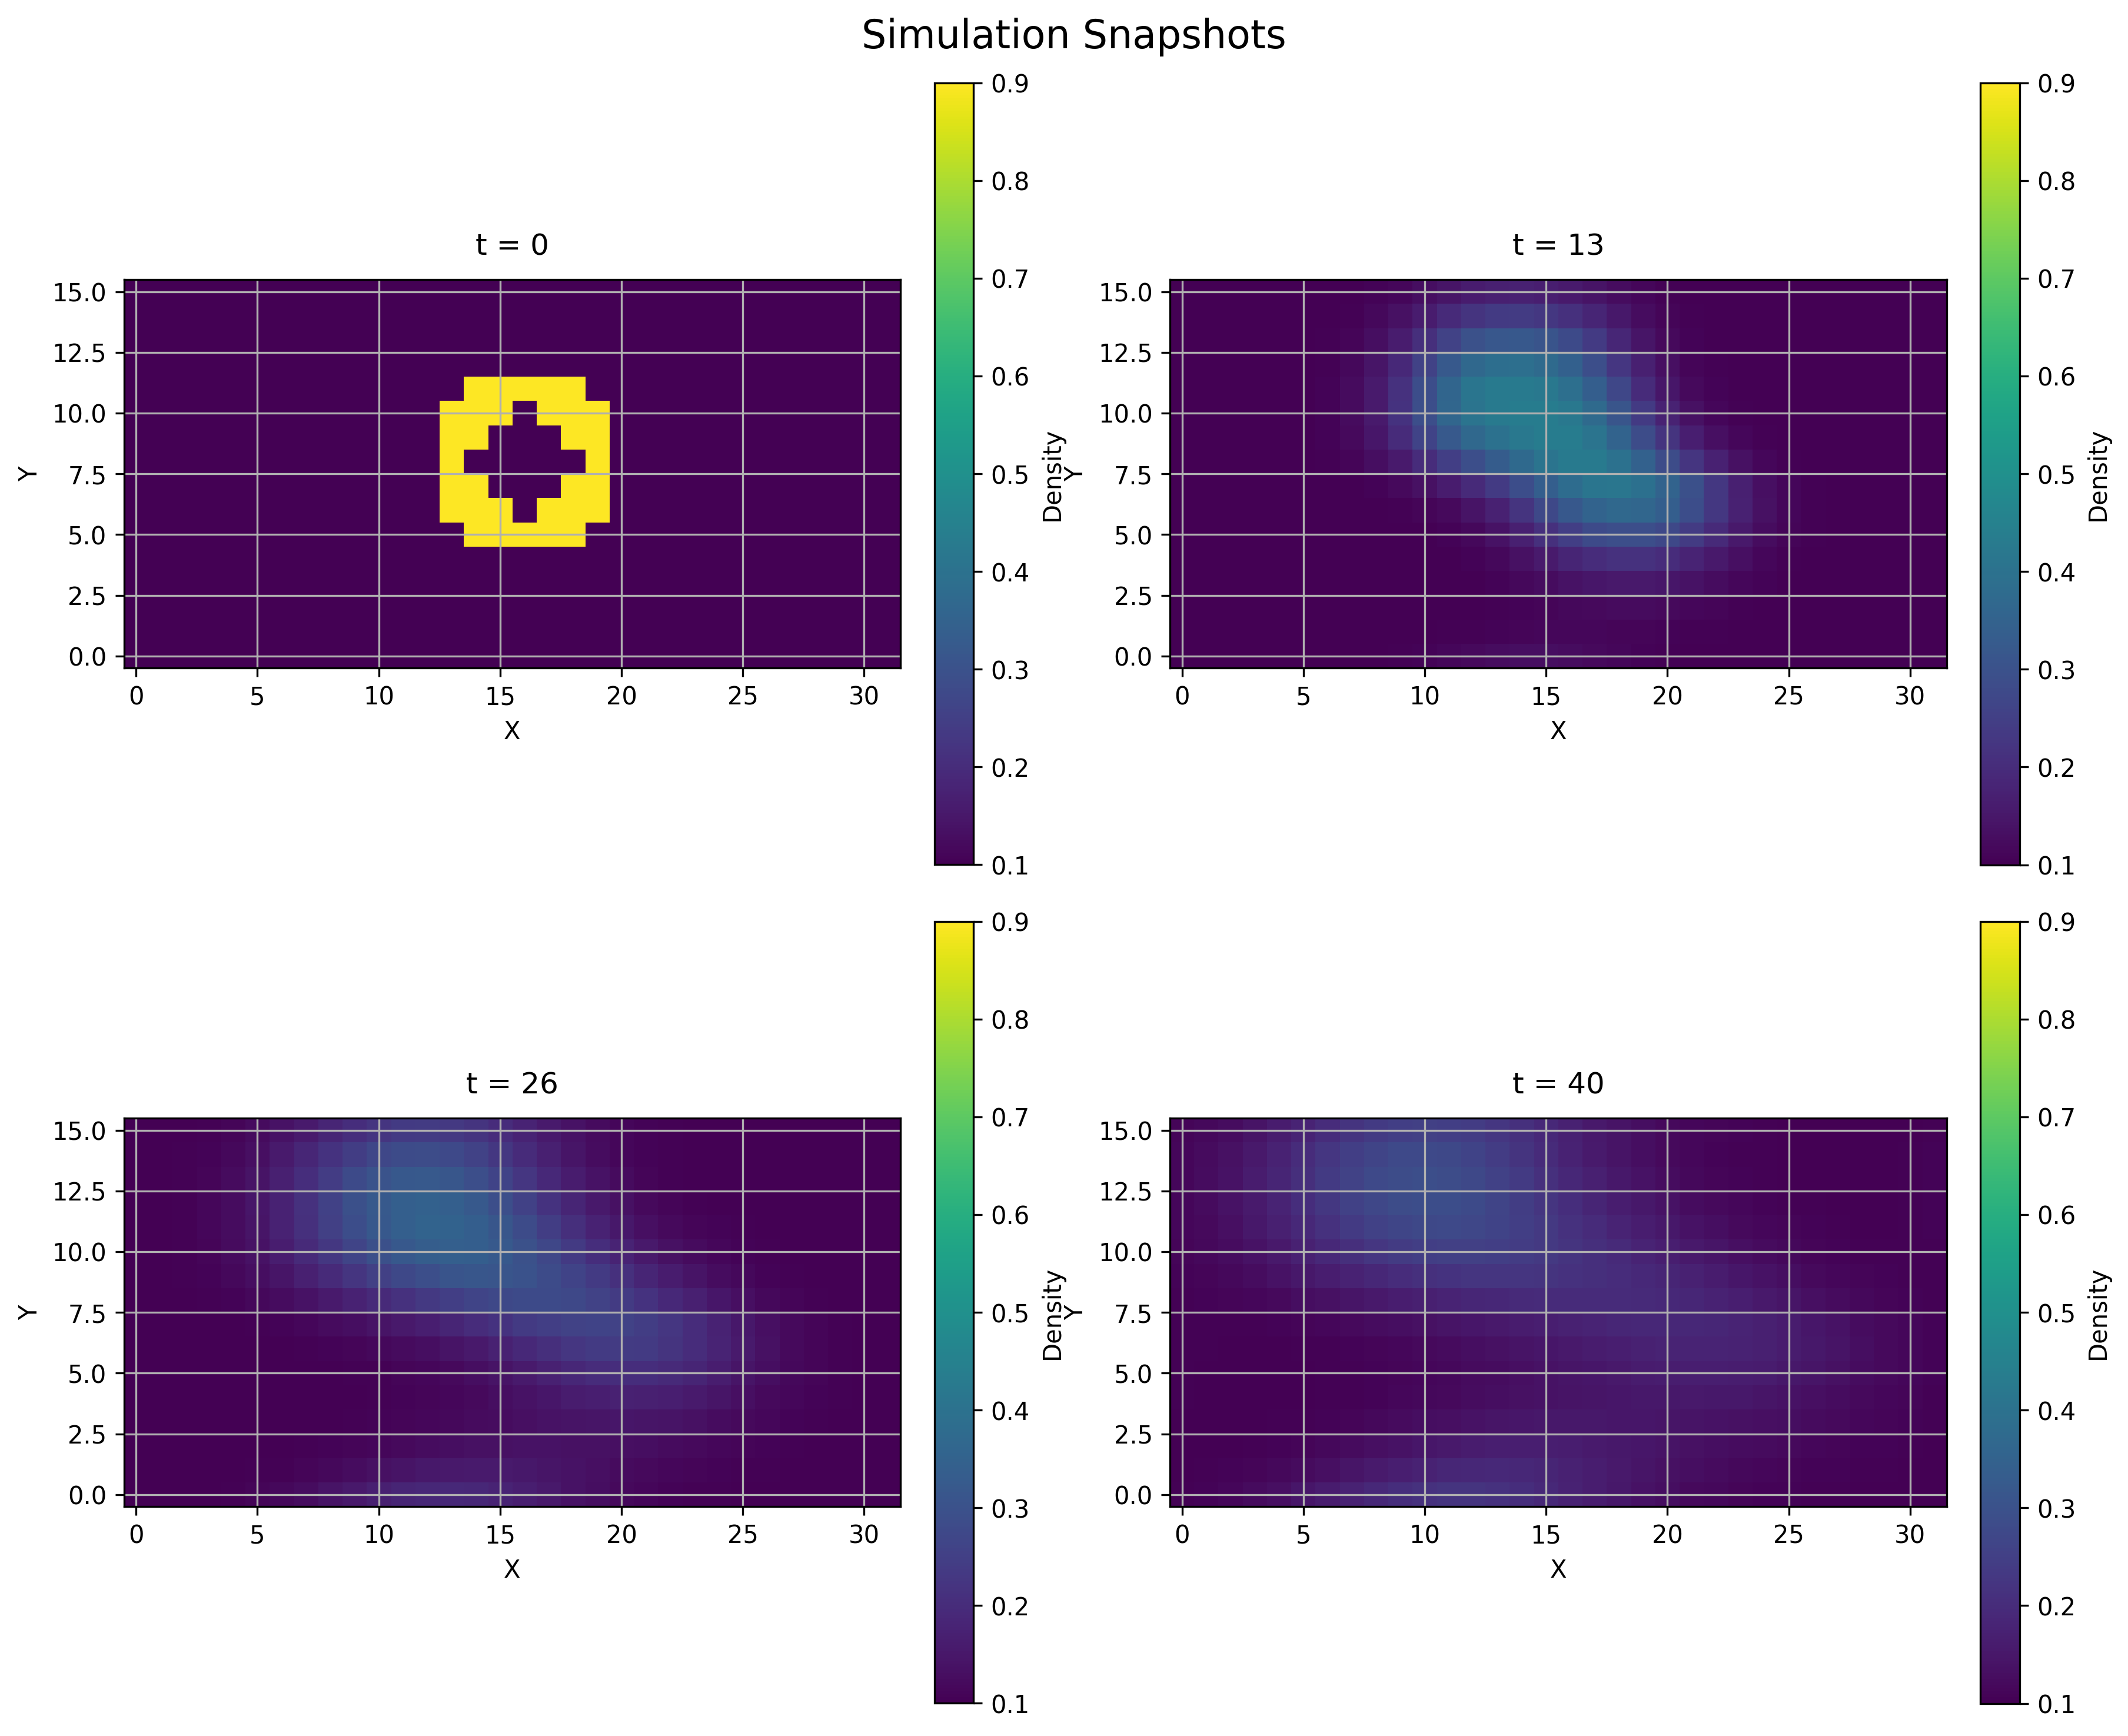
\includegraphics[height=0.5\textheight]{2_Dquantum}
    \end{column}
    \begin{column}{0.5\textwidth}
      \centering
      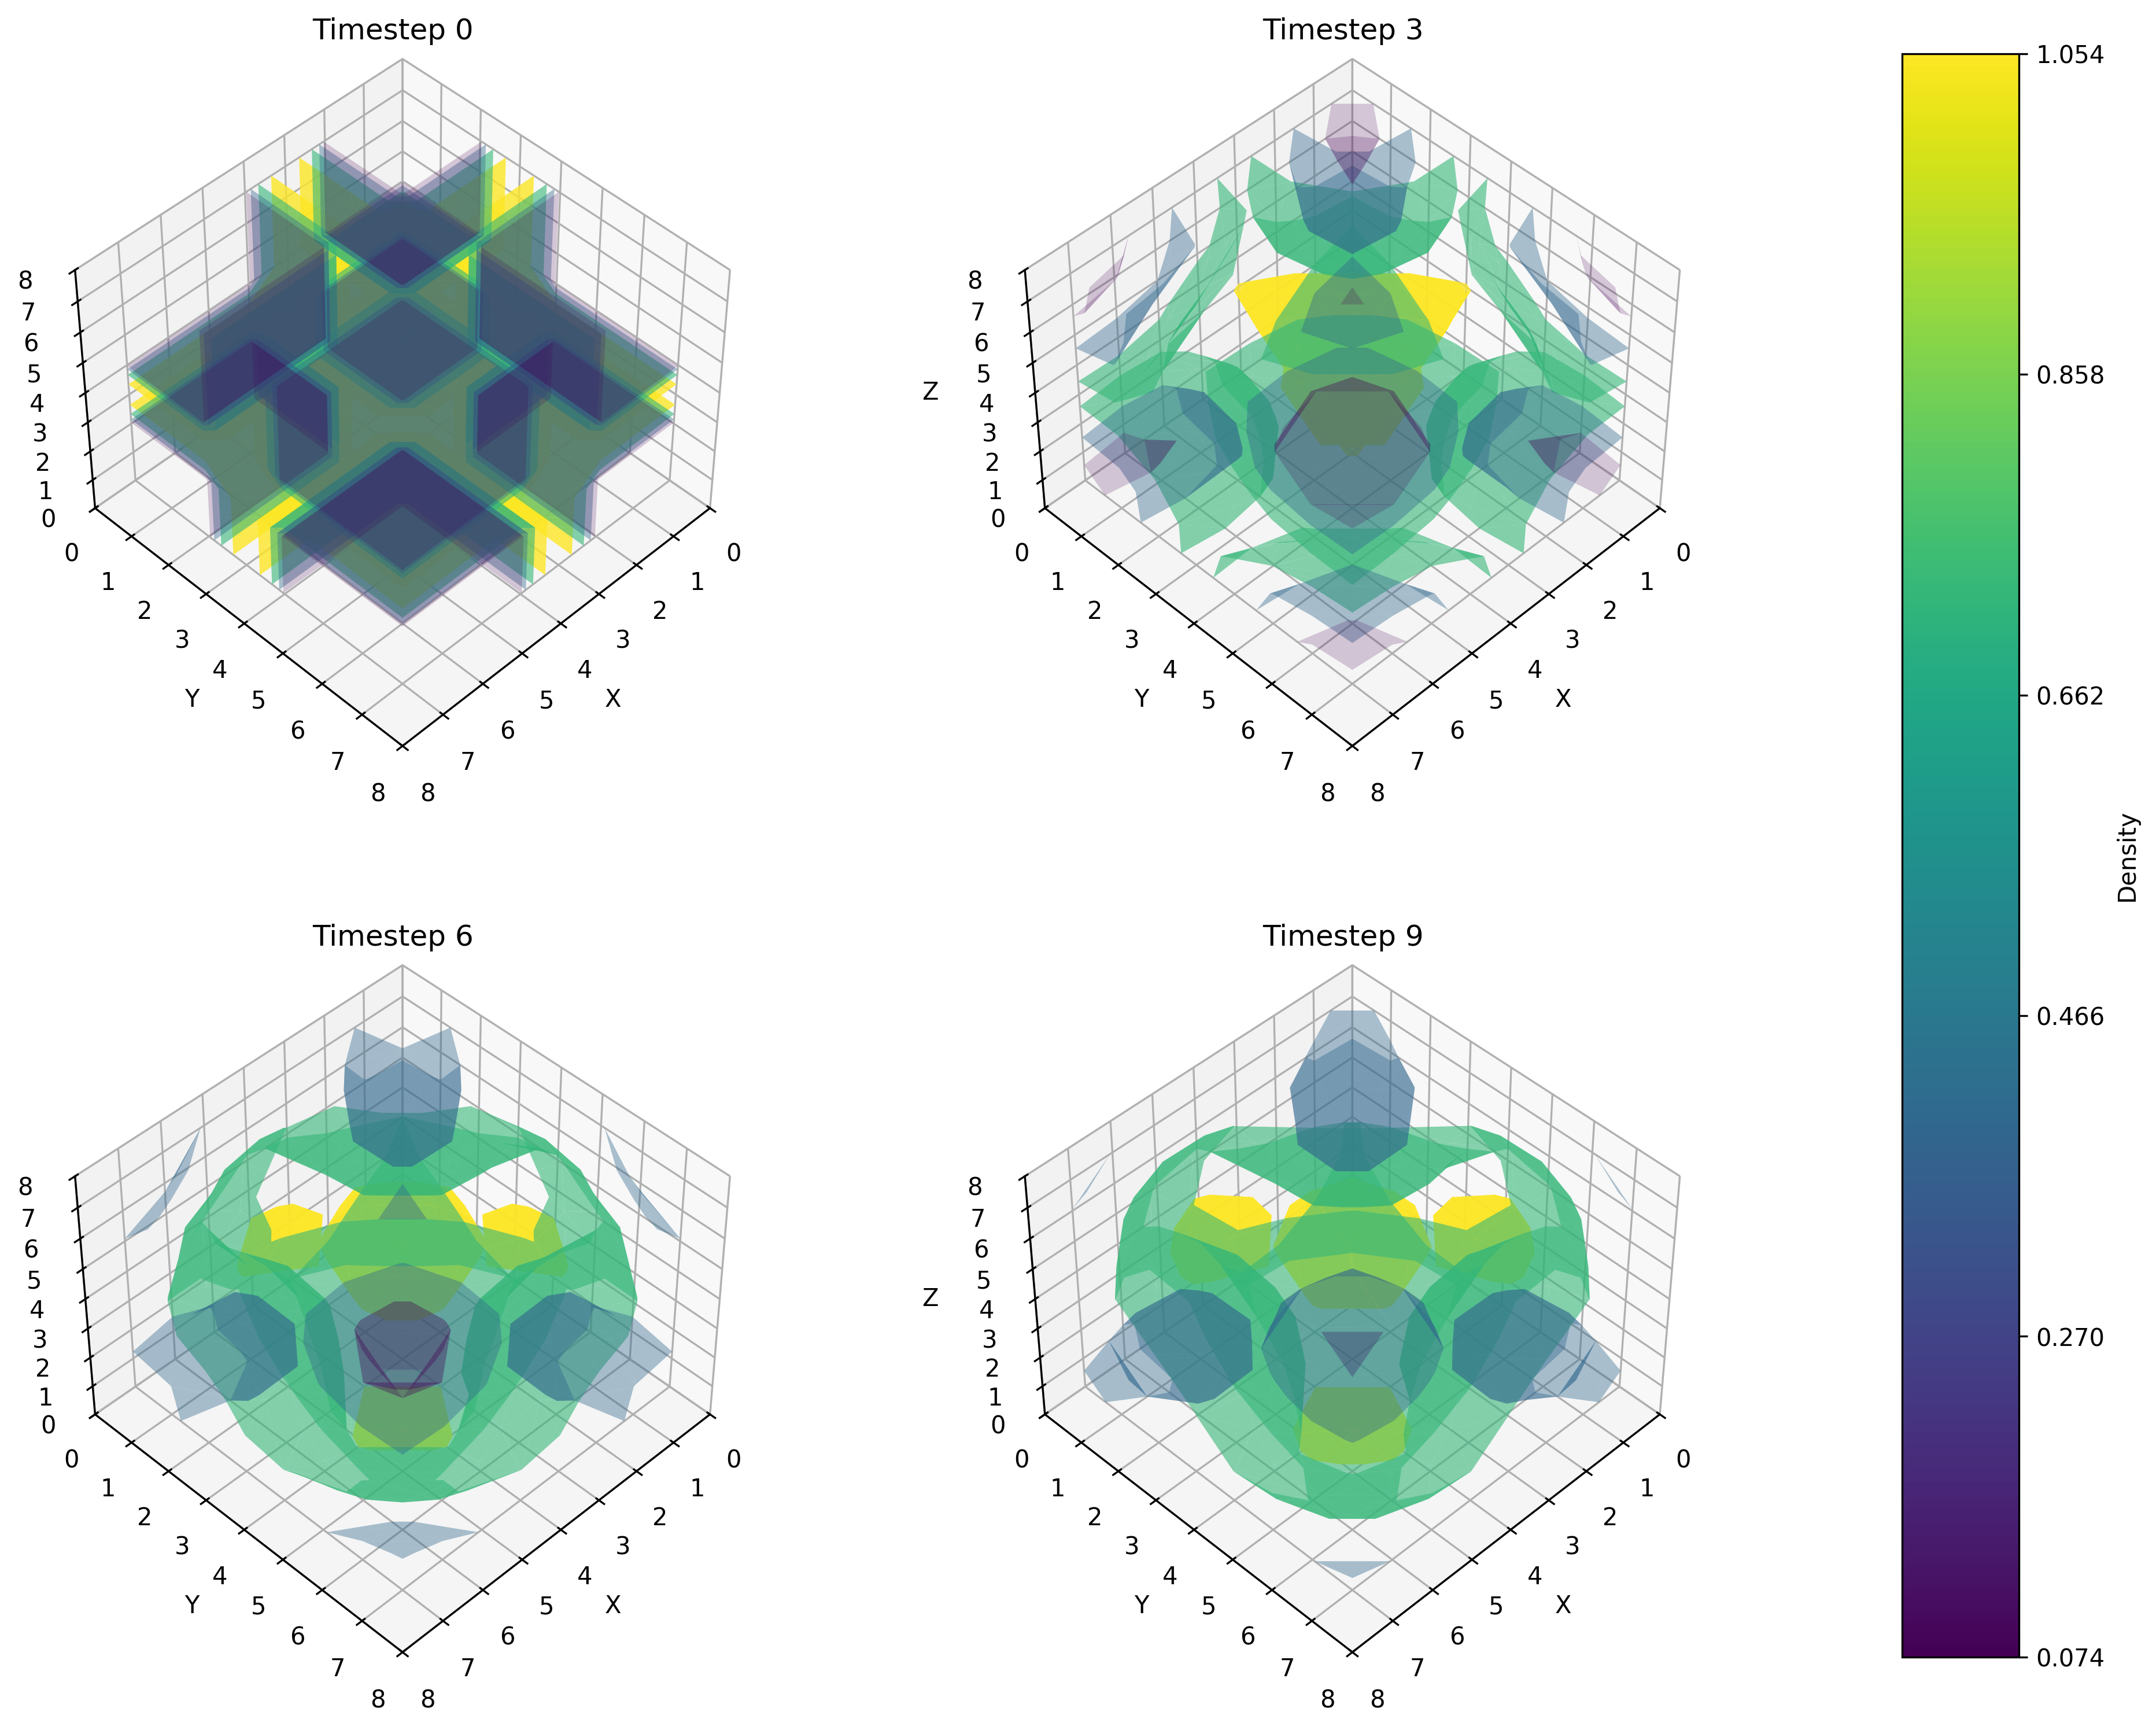
\includegraphics[height=0.5\textheight]{3_Dquantum_snapshots}
    \end{column}
  \end{columns}
  \vspace{0.3em}
  \centering
  {\small Matches the classical reference across 1D, 2D and 3D.}
  \note{With the implementation, I could both validate the correctness and reproduce
  literature results.}
\end{frame}

\begin{frame}{Performance}
  \begin{columns}[c]
    \begin{column}{0.5\textwidth}
      \centering
      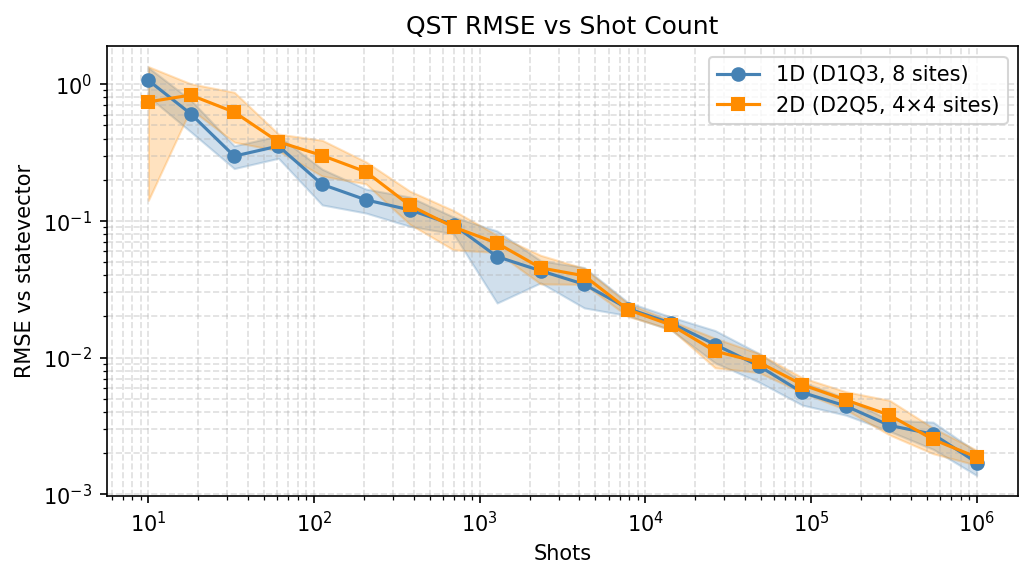
\includegraphics[height=0.5\textheight]{qst_rmse}\\
      {\small State tomography: $\sim 10^{6}$ shots per iteration.}
    \end{column}
    \begin{column}{0.5\textwidth}
      \centering
      {\footnotesize Transpiled gates / circuit depth\\[0.4em]
      \begin{tabular}{lcc}
        \toprule
        Configuration & Gates & Depth \\
        \midrule
        D1Q3 $M{=}16$     & 3{,}694  & 2{,}680 \\
        D2Q9 $8{\times}8$ & 41{,}027 & 29{,}544 \\
        D3Q27 $4{\times}4{\times}4$ & 66{,}456 & 49{,}116 \\
        \bottomrule
      \end{tabular}}\\[0.5em]
      {\small Deep circuits, even for small lattices.}
    \end{column}
  \end{columns}
  \vspace{0.5em}
  \centering
  {\small Far from practical on near-term quantum computers.}
  \note{I personally did not find satisfying performance experiments in the literature,
  especially on the impact of quantum state tomography, so I did my own. Without getting
  into the numbers, my experiments and analysis showed that this particular algorithm is
  far from being practical on near-term quantum computers, so further improvements will
  be needed.}
\end{frame}

\begin{frame}{Boundary conditions}
  \vfill
  \centering
  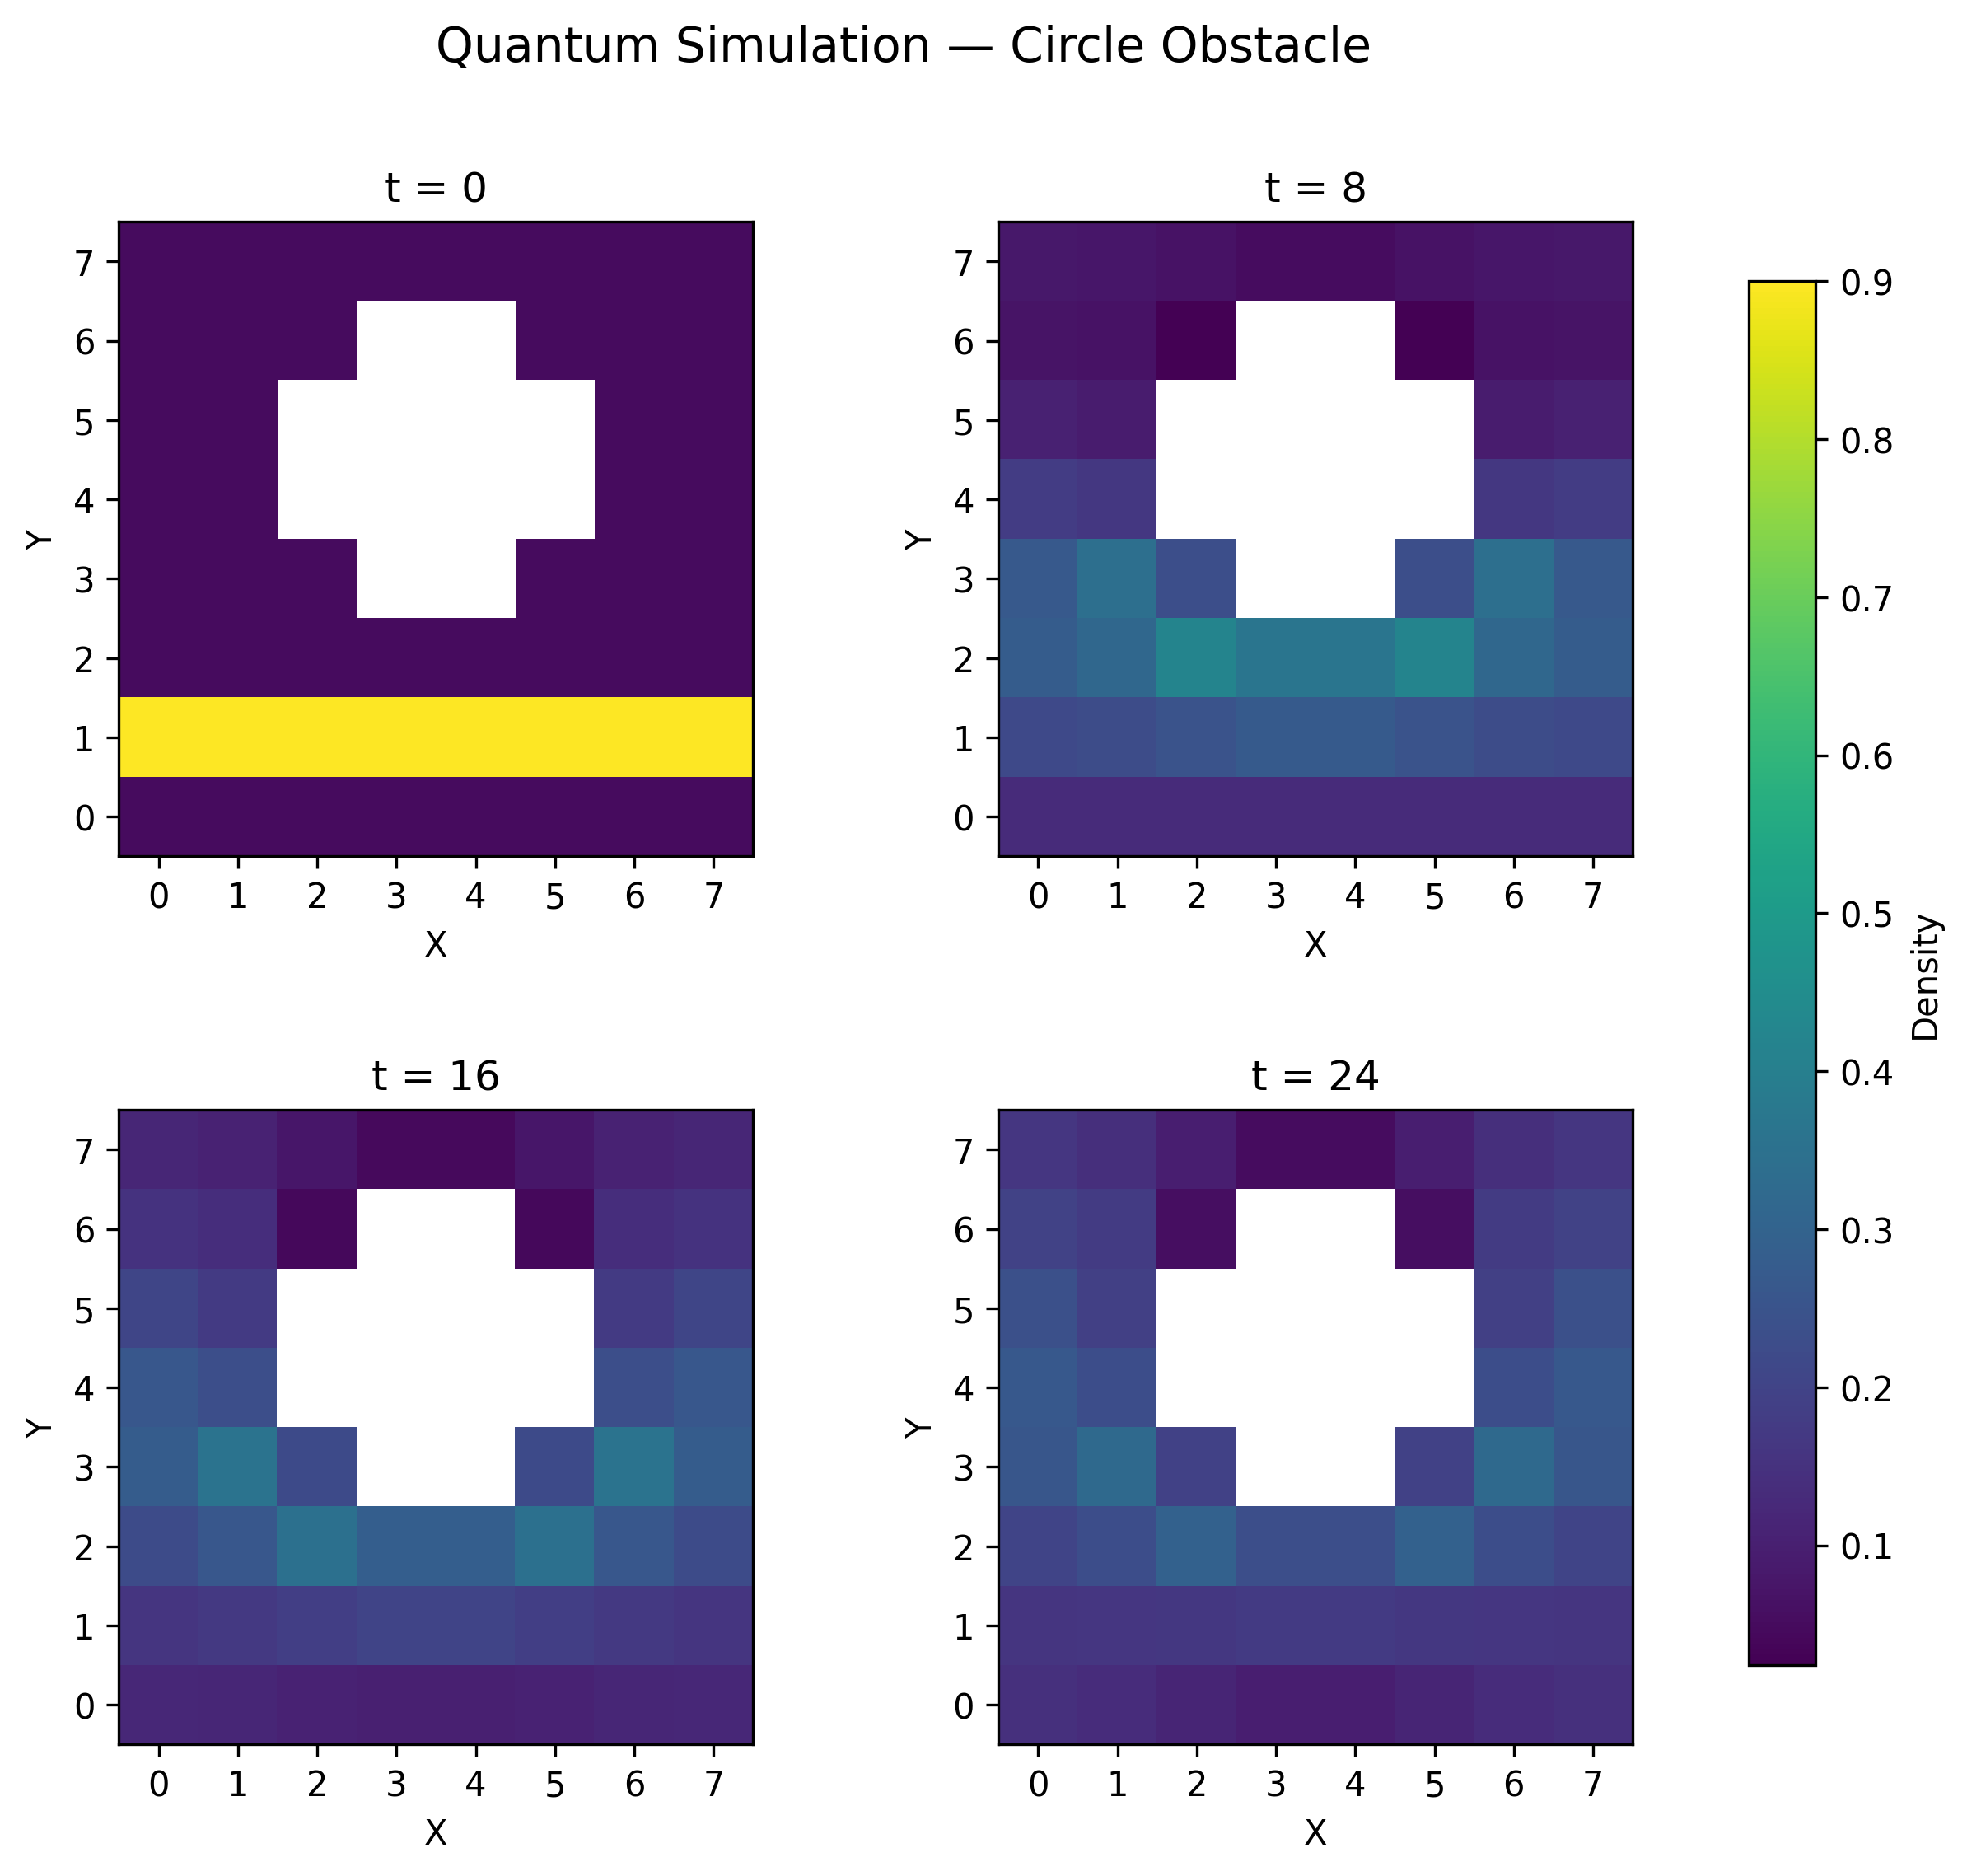
\includegraphics[height=0.55\textheight]{bc_2d_snapshots}
  \\[0.4em]
  {\small Rules for the fluid at walls and obstacles.}
  \vfill
  \note{Next up, I attempted my own original contribution to the underlying algorithm, in
  the form of a flexible method for defining a large class of boundary conditions. Now,
  what are boundary conditions? They are concrete rules for how the fluid should behave in
  certain areas, such as the edges of the simulation or other obstacles. For example,
  solid walls preventing fluid flow.}
\end{frame}

\begin{frame}{A flexible formulation}
  \vfill
  \centering
  A linear system per node, redistributing the populations:
  \[ \mathbf{f}^{post}(x) = B_x\,\mathbf{f}^{pre}(x) \]
  with the only restriction that the total quantity is preserved:
  \[ \textstyle\sum_i f_i^{post} = \sum_i f_i^{pre}. \]
  \vfill
  \note{My idea was to define, for each node, a linear system of equations governing the
  redistribution of the populations. The only restriction being that the total fluid
  quantity should be preserved. I later discovered this was far from a new idea in the
  classical world, but I never saw it applied to the quantum variant.}
\end{frame}

\begin{frame}{Combining the operators}
  \vfill
  \centering
  \large
  The boundary matrix is non-unitary again $\rightarrow$ another LCU.
  \\[1em]
  Two consecutive LCUs: the failure probabilities compound.
  \\[1.2em]
  {\color{mOrange} Idea: merge collision and boundary conditions into one matrix,
  a single LCU.}
  \vfill
  \note{Yet again, the matrix encoding the system is generally not unitary, so I just used
  LCU to apply it. Now, you might notice an issue in applying two consecutive LCUs: the
  failure probabilities compound. To fix this, I thought of combining the collision and
  boundary condition operators into a single matrix and only performing LCU on that one.}
\end{frame}

\begin{frame}{Two caveats}
  \vfill
  \centering
  Moving the boundary conditions before streaming stays equivalent:
  \[ B_{pre} = S^{\dagger} B_{post} S \]
  And the merged circuit never does worse:
  \[ P_{merged} \;\ge\; P_{separate} \]
  \vspace{0.3em}
  {\footnotesize
  \begin{tabular}{lcc}
    \toprule
    Configuration & $P_{merged}$ & $P_{separate}$ \\
    \midrule
    D1Q3 $N{=}4$      & 0.37 & 0.23 \\
    D1Q3 $N{=}8$      & 0.27 & 0.16 \\
    D2Q5 $4{\times}4$ & 0.31 & 0.23 \\
    \bottomrule
  \end{tabular}}
  \vfill
  \note{There were two issues to overcome. First, we had to move the boundary conditions
  to before streaming, which makes their physical meaning incorrect; fortunately, it is
  relatively easy to prove that for any post-streaming boundary matrix there is a mapping
  to an equivalent pre-streaming matrix. The second issue was whether this actually
  improved the success probability; as it turns out, I could mathematically prove that the
  combined matrix's success probability is always at least as good as doing them
  separately.}
\end{frame}

\begin{frame}{Validation and cost}
  \begin{columns}[c]
    \begin{column}{0.5\textwidth}
      \centering
      {\small Correct against the classical reference,\\ but inefficient in its current form.}
    \end{column}
    \begin{column}{0.5\textwidth}
      \centering
      {\footnotesize Transpiled gate count\\[0.3em]
      \begin{tabular}{lccc}
        \toprule
        Config & Coll. & Coll.+BC & $\times$ \\
        \midrule
        D1Q3 $M{=}8$  & 786   & 9{,}451   & $12\times$ \\
        D1Q3 $M{=}16$ & 1{,}563 & 38{,}380 & $25\times$ \\
        D1Q3 $M{=}32$ & 3{,}110 & 154{,}605 & $50\times$ \\
        \bottomrule
      \end{tabular}}
    \end{column}
  \end{columns}
  \note{Once again, I validated the correctness against a classical implementation and
  analyzed the performance impact of my addition. The results showed that, while correct,
  my approach was highly inefficient in its current form. Further improvements must be made
  before it is anywhere near practical.}
\end{frame}

% =====================================================================
%  Demo
% =====================================================================
\begin{frame}[plain]
  \vfill
  \centering
  {\usebeamercolor[fg]{title}\Huge\bfseries Live Demo}\\[0.8em]
  {\large 1D advection-diffusion with boundary conditions}
  \vfill
  \note{Now I have a short demo for a 1D example experiment with boundary conditions. I have
  chosen the 1D case because it is simple to modify and runs relatively fast.}
\end{frame}

% =====================================================================
%  Conclusions
% =====================================================================
\section{Conclusions}

\begin{frame}{Conclusions}
  \vfill
  \begin{itemize}
    \item Existing QLBM algorithms have key limitations that must be overcome before they are useful.
    \item I experimented with an original extension supporting parametrized boundary conditions.
  \end{itemize}
  \vfill
  \note{In conclusion, my research shows that the existing quantum algorithms for the
  Lattice Boltzmann Method have key limitations that must be overcome before they can be of
  any use. Additionally, I also experimented with an original extension to the algorithm in
  order to support parametrized boundary conditions.}
\end{frame}

\begin{frame}[plain]
  \vfill
  \centering
  {\usebeamercolor[fg]{title}\Huge\bfseries Thank you}\\[0.8em]
  {\large Questions?}
  \vfill
  \note{And this concludes my presentation. I am eager to hear your questions.}
\end{frame}

\end{document}
